
\begin{figure}
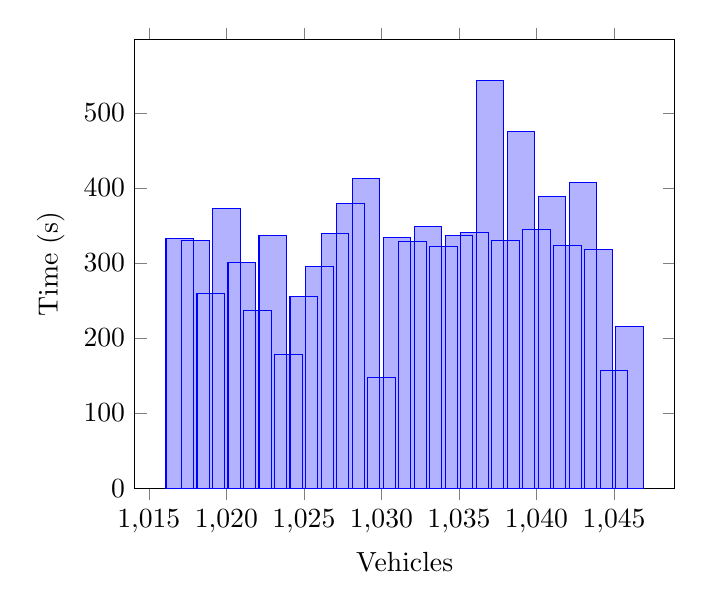
\begin{tikzpicture}
\begin{axis}[
legend style={anchor=west},
xlabel=Vehicles,
ylabel=Time (s),
ymin=0,
ybar,
]
\addplot coordinates {
(1043, 407)
(1034, 322)
(1019, 259)
(1028, 379)
(1040, 344)
(1044, 318)
(1035, 336)
(1021, 300)
(1039, 475)
(1020, 372)
(1026, 295)
(1030, 147)
(1023, 337)
(1017, 333)
(1038, 330)
(1042, 323)
(1045, 157)
(1041, 388)
(1033, 349)
(1018, 330)
(1024, 178)
(1027, 339)
(1046, 215)
(1022, 237)
(1031, 334)
(1029, 412)
(1032, 329)
(1037, 543)
(1036, 340)
(1025, 255)
};

\end{axis}
\end{tikzpicture}
\label{tik:time:0:96}
\caption{0 percent diving with GSC on route $96$}
\end{figure}
